\chapter{Wireframe}

\begin{figure}[h]
    \centering
    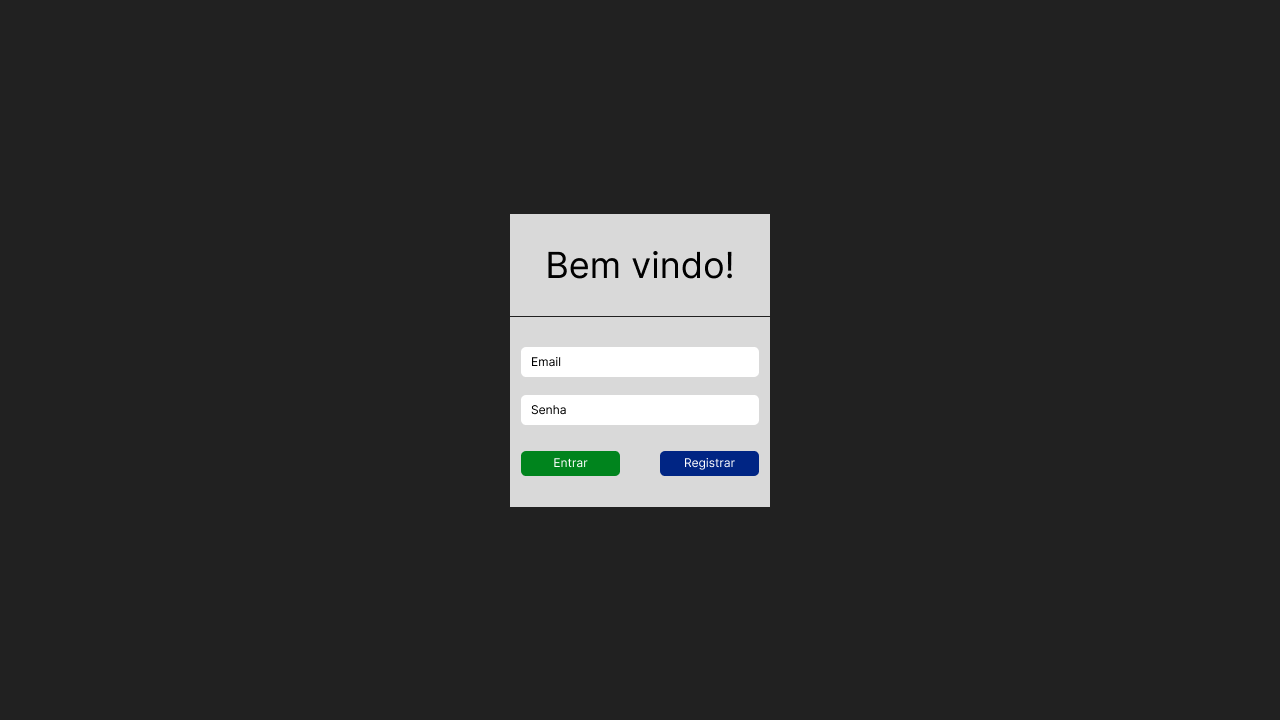
\includegraphics[width=1\textwidth]{../figures/login.png}
    \caption{Tela de login}
    \label{fig:login}
\end{figure}

\begin{figure}[h]
    \centering
    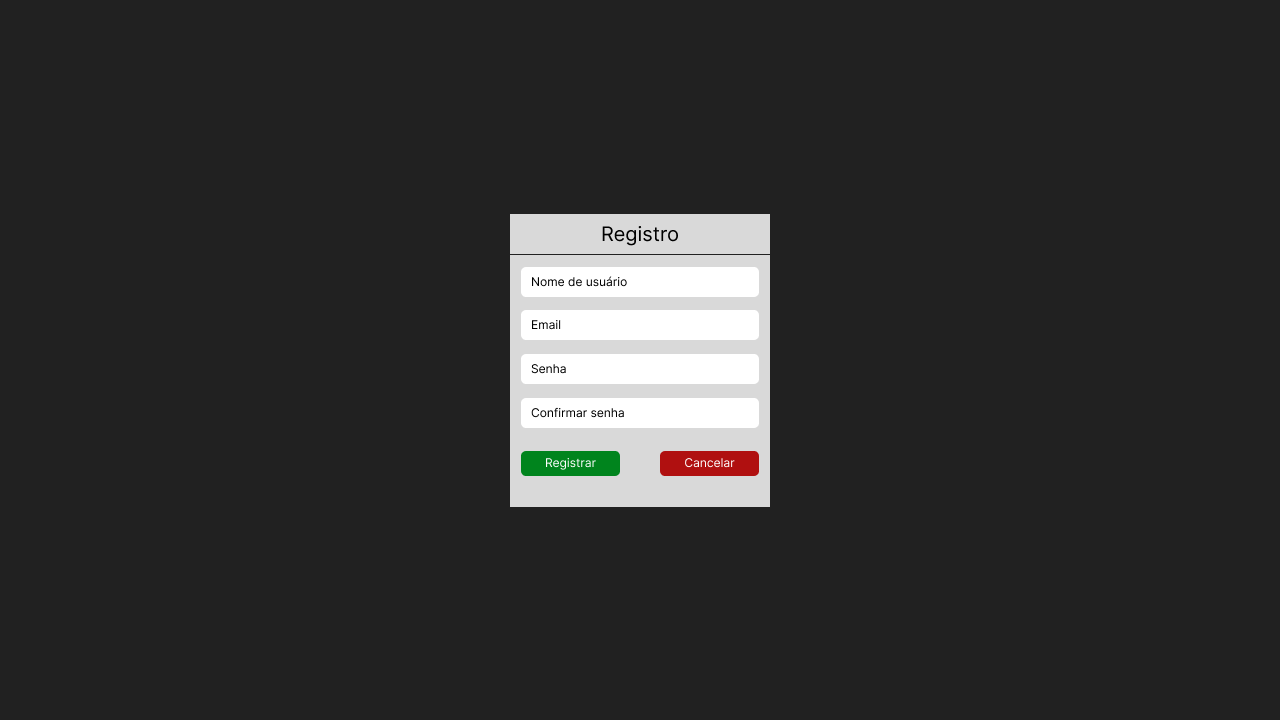
\includegraphics[width=1\textwidth]{../figures/registrar.png}
    \caption{Tela de registro de usuário}
    \label{fig:registrar}
\end{figure}

\begin{figure}[h]
    \centering
    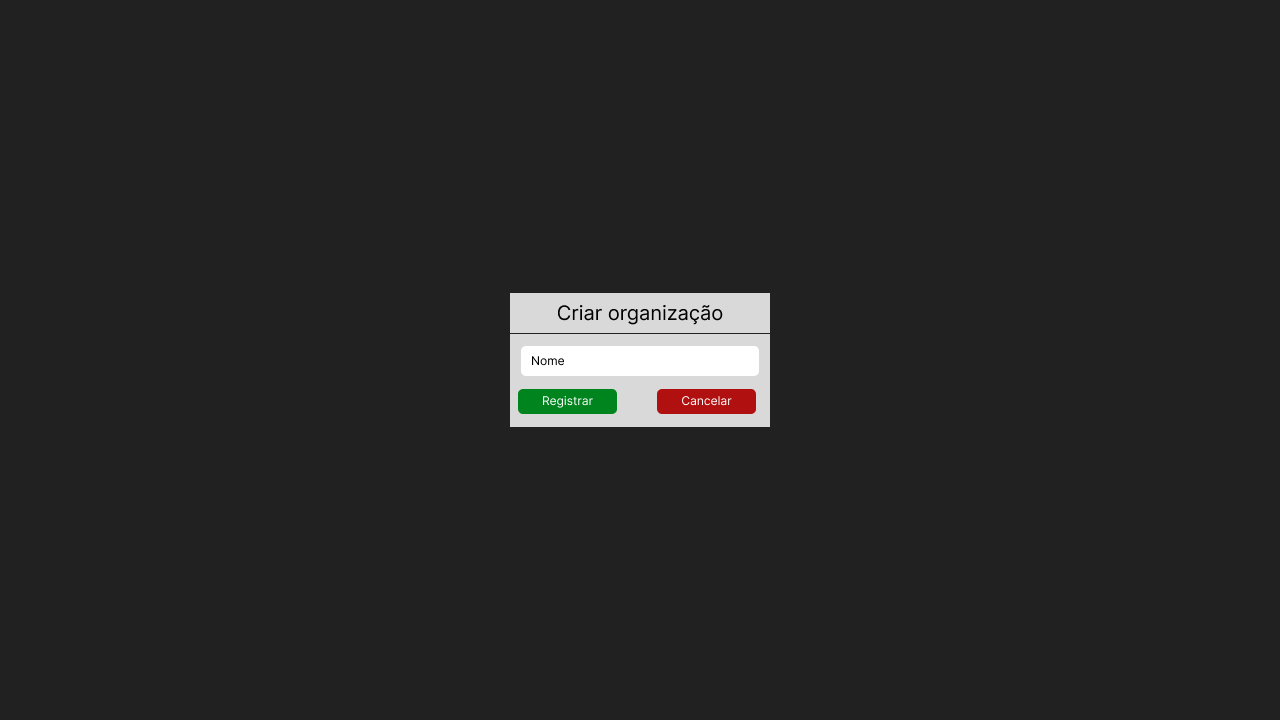
\includegraphics[width=1\textwidth]{../figures/criar-organizacao.png}
    \caption{Tela de criar organização}
    \label{fig:criar-organizacao}
\end{figure}

\begin{figure}[h]
    \centering
    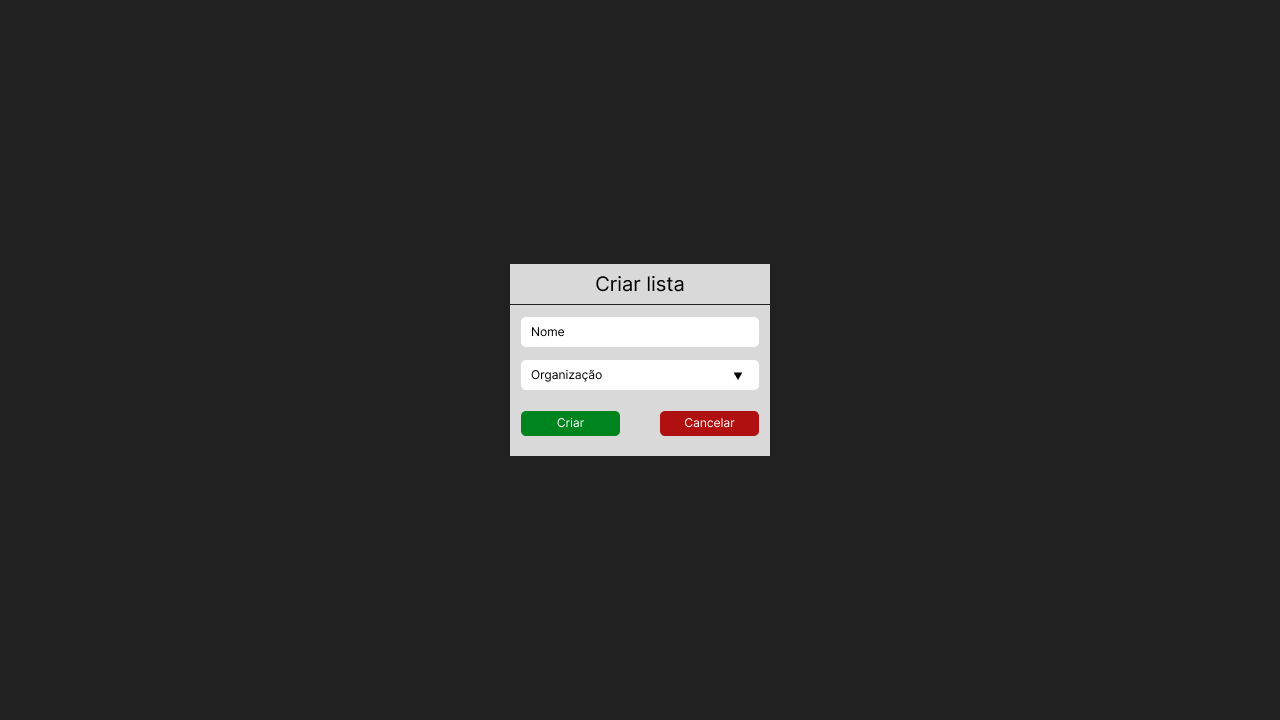
\includegraphics[width=1\textwidth]{../figures/criar-lista.png}
    \caption{Tela de criar lista de tarefas}
    \label{fig:criar-lista}
\end{figure}

\begin{figure}[h]
    \centering
    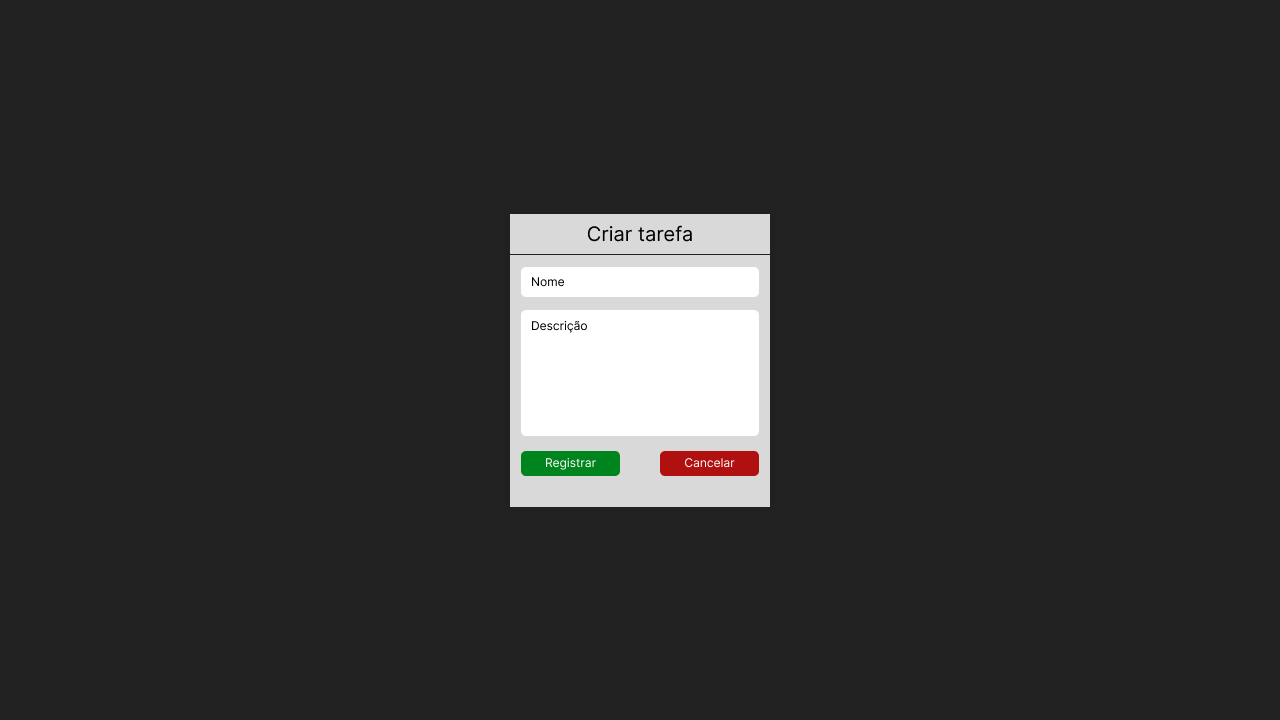
\includegraphics[width=1\textwidth]{../figures/criar-tarefa.png}
    \caption{Tela de criar tarefas}
    \label{fig:criar-tarefa}
\end{figure}